\chapter{Implementation of an IoT based Electronic Voting Machine}

\section{Hardware and software setup}
\begin{table}[h!]
    \centering
    \begin{tabular}{|l|c|p{5cm}|}
        \hline
        \textbf{Device} & \textbf{Number} & \textbf{Notes} \\
        \hline
        ESP32 & 2 & NodeMCU Dev. Board \\
        \hline
        Laptop & 1 & Sony Vaio VPCEH3G1E \\
        \hline
    \end{tabular}
    \caption{Hardware devices}\label{tab:hardware-components}
\end{table}

\begin{figure}
	\centering
	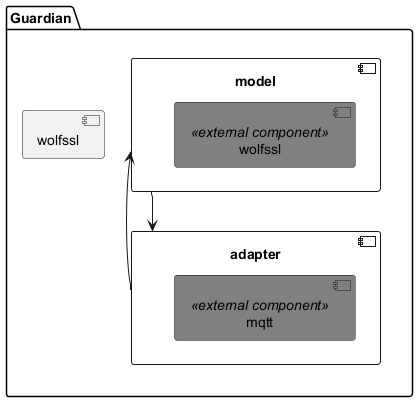
\includegraphics[scale=.5]{abbildungen/Diagramme/components.png}
	\caption{Software components for the Guardian Prototype}\label{Fig:software-components} 
\end{figure}

The hardware configuration is presented in Table \ref{tab:hardware-components}, providing a detailed account of the devices involved in the experimental setup. The laptop and the ESP32 devices are connected via wi-fi 


The NodeMCU ESP32 development board serves as the main controller, while the LCD display module is used to present information to the user. The button module allows user interaction, and the jumper wires are used to connect the components. The breadboard is used to build the circuits. 

Figure \ref{Fig:software-components} depicts the software components used in the Guardian Prototype. The software components model contains the business logic, the adapter component includes the communication logic, and the view component is responsible for the user interface.

\begin{figure}
	\centering
	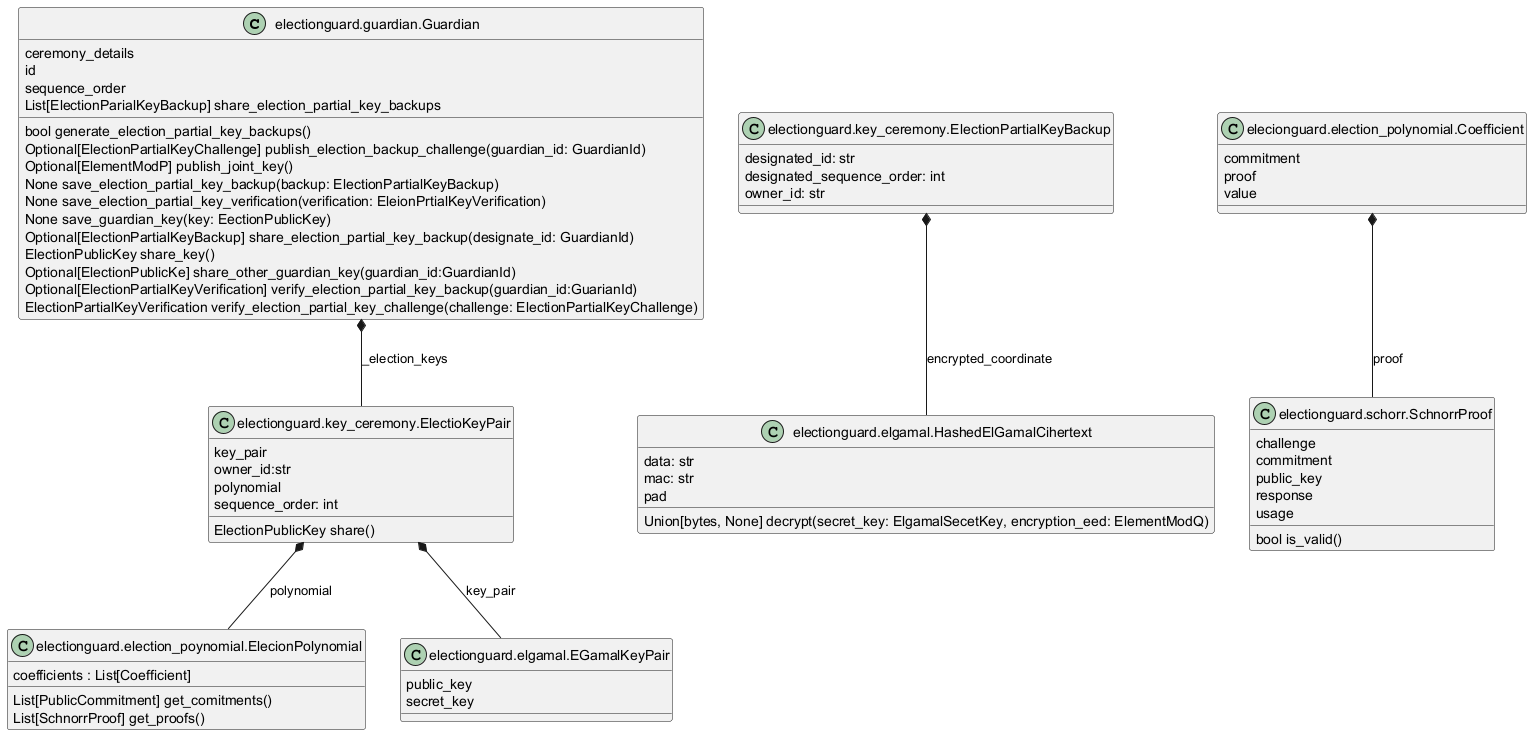
\includegraphics[scale=.7]{abbildungen/Diagramme/python-classes.png}
	\caption{Python Classes}\label{Fig:python-class} 
\end{figure}

The model component implements the ElectionKeyPair and ElectionPartialKeyBackup classes from the python reference implementation as seen in figure as c structs \ref{Fig:python-class} the c structs can be found in Appendix \ref{lst:structs} 

. These classes are based from the python classes as seen in Figure \ref{Fig:python-class}. 




The hardware configuration is presented in Table \ref{tab:basic-component-list}, providing a detailed account of the devices involved in the experimental setup. Table \ref{tab:software} contains the specific software tools and applications pivotal to this research.



\subsection{Algorithms}


\begin{comment}
For considering the communication scope, we reviewed
the current state-of-art literature to identify the IoT
communication types based on environments running IoT
applications.
Device-to-Device (D2D) where communication is
provided between two nodes or devices directly.
Device-to-Device (D2D) where communication is
provided between two nodes or devices directly.
Device-to-Gateway (D2G) where communication is
provided through a gateway that resides in close
proximity to the edge of the network while interacting
with IoT devices. \cite[6]{protocols}

    There are a number of MQTT model implementations
including Mosquitto, eMQTT, HiveMQ, Moquette, among
many others. \cite[10]{protocols}



As shown in Table \ref{tab:basic-component-list}, the hardware components used in our prototype include a ESP32 development board, an LCD display module, jumper wires, breadboard and a module with 2 Buttons. The connectivity of these components are shown in the schematic in Figure \ref{Fig:schematic}. The NodeMCU ESP32 development board is used as the Main Controller. The LCD display module is used to display information to the user. The button module is used to interact with the user. The jumper wires are used to connect the components. The breadboard is used to build the circuits.

\subsection{NodeMCU ESP32 Development Board}
The NodeMCU ESP32 development board is equipped with the ESP32-WROOM-32 module. 

\subsection{1,8" LCD Display Module}
The 1,8" LCD Display Module has a resolution of 128x160 Pixels and is equipped with a ST7735R Display Driver.  The module also contains a microSD Slot which won't be used in this project \cite[2]{lcd}.

\subsection{Button Module}
The Button Module is an integrated circuit that features 2 buttons and integrated pull-up resistors. \cite[1]{button-ds}

\section{Python Client}
Our python client imports the python package ElectionGuard \cite{python-reference}. The ElectionGuard Python package is a reference implementation of the ElectionGuard 1.0 specification. It covers the entire suite of functionality required to implement an end-to-end verifiable election as part of a voting system \cite{eg-docs}. 



In the proposed voting system the python client will act as the administrator, the ballot box and the encryption device of the election. Administrating the election requires loading and semantically verifiying the Election manifest before the election.





Before the election the python client load the Election Manifest for our election and semantically checks the data format required to conduct an ElectionGuard Election. 




The python client loads the manifest file used for our election. In ElectionGuard an election manifest has to be semantically checked against the data format required to conduct an ElectionGuard Election. 


The python client then generates the election keys and the election context. The election keys are used to encrypt the ballots and the election context is used to verify the election. The python client then encrypts the ballots and generates the proofs of the encryption. The encrypted ballots and the proofs are then sent to the ESP32. The ESP32 decrypts the ballots and verifies the proofs. The ESP32 then generates the proofs of the decryption and sends them back to the python client. The python client then verifies the proofs of the decryption and generates the proofs of the election. The proofs of the election are then sent to the ESP32. The ESP32 verifies the proofs of the election and sends the results back to the python client. The python client then verifies the results and outputs the final results of the election.

The tasks of the python client can be divided into three stages pre-election, intra-election and post-election.







The python client loads the manifest file used for our election. In ElectionGuard an election manifest has to be semantically checked against the data fromat required to conduct an ElectionGuard Election.



Espressif IoT Development Framework (ESP-IDF) is a software development framework intended for the development of Internet-of-Things (IoT) applications for the ESP32 board \cite{esp-prog}. ESP-IDF consists of components written specifically for ESP-IDF as well as third-party libraries.\cite{esp-prog} For example, the real-time operating system kernel used for ESP-IDF applications is the third-party component called FreeRTOS \cite{esp-prog}. ESP-IDF projects use the same componment based approach and can be seen as an amalgamation of a number of components \cite{esp-prog}.

\begin{figure}
	\centering
	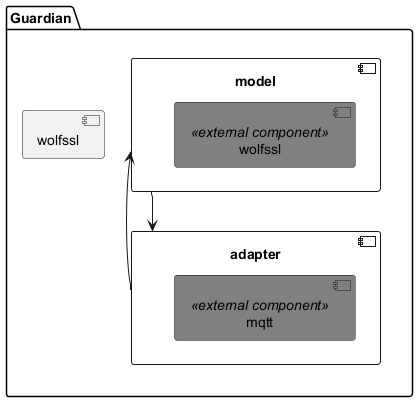
\includegraphics[width=1\textwidth]{abbildungen/Diagramme/components.png}
	\caption{}
	\label{Fig:uml-classes-python}
\end{figure}

\end{comment}




\section{Computation}
ElectionGuard uses integer ElGamal cryptography within its specific cryptographic operations. The system performs four key operations on very large integer values: \textbf{modular exponentiation}, \textbf{modular multiplication}, \textbf{modular addition}, and \textbf{SHA-256} hash computation. To handle the large integer values involved in these operations, specialized libraries for large integers may be employed, or the operations can be developed from scratch \cite[21, 25-26]{eg-spec}. When developing these modular operations from the ground up, it is common for intermediate values to become excessively large. Techniques such as modular reduction are often necessary to ensure that values remain manageable \cite[21, 25-26]{eg-spec}.Consequently, employing optimized libraries for modular arithmetic becomes crucial for achieving good performance \cite[22]{eg-paper}.

\subsection{Cryptographic constants}
Among all computations in ElectionGuard, modular exponentiation presents the highest computational cost, serving as the primary limiting factor in performance analysis \cite[22]{eg-spec}. Within ElectionGuard, most modular exponentiation operations utilize a fixed base, which may be either the generator (g) or a public key \cite[22]{eg-paper}. The generator G is a mathematical constant specified in the ElectionGuard specification.

The standard baseline parameters include:
\begin{itemize}
    \item A 4096-bit prime (p) \cite[22]{eg-spec}
    \item A 4096-bit generator (g) \cite[23]{eg-spec}
    \item A 256-bit prime (q) \cite[21]{eg-spec}
\end{itemize}

Alternatively, the system can also utilize reduced baseline parameters, which consist of:
\begin{itemize}
    \item A 3072-bit prime (p) \cite[36]{eg-spec}
    \item A 3072-bit generator (g) \cite[36-37]{eg-spec}
    \item A 256-bit prime (q) \cite[36]{eg-spec}
\end{itemize}

For this application, we opt for the reduced parameters, as they offer enhanced performance, albeit at the expense of lower security \cite[36-37]{eg-spec}. The cryptographic constants used in the implementation can be found in Appendix \ref{lst:constants}.



\subsection{Comparison of ElectionGuard Implementations}
The Python reference implementation of ElectionGuard utilizes the C-coded Gmpy2 library for large integer arithmetic. In contrast the C++ and Kotlin implementations rely on the HACL* C library for similar purposes \cite{eg-docs}. Interestingly, both implementation use C-coded libraries for handling large integer arithmetic. Moreover, the C++ implementation incorporates pre-computed tables to speed up certain modular exponentiations \cite{eg-docs}. This optimization is possible because many of the exponentiations are performed with a fixed base, either the constant generator (g) or a public key. The pre-computed tables contain specific powers of these bases \cite{eg-docs}.

\subsubsection{Feasability of the Python reference on ESP32}
The Python reference implementation encompasses the entire ElectionGuard specification \cite{python-reference}. Running the Python reference implementation on the ESP32 may be achievable through \textbf{MicroPython}, an implementation of Python 3.x targeted for microcontrollers and embedded systems. MicroPython mirrors and adapts the functionalities of the standard Python library to accommodate the limitations inherent to to microcontrollers, such as restricted memory and processing speed \cite{micropython} \cite[234]{micropython-performance}. There are drawbacks to this approach, as certain essential modules, functions, and classes may be absent in MicroPython \cite{micropython}. Additionally, applications developed in MicroPython are prone to memory fragmentation and may experience issues with objective expending in size. \cite[234]{micropython-performance}. Depending on the complexity of the task and memory allocation, the performance of MicroPython might be inferior to that of a C implementation \cite[237]{micropython-performance}. For instance, in a comparative study of software-based SHA-256 computation for the ESP32, the C implementation outperformed the MicroPython implementation by 45\% \cite[237]{micropython-performance}.

\subsubsection{Feasability of the C++ reference on ESP32}
The ElectionGuard C++ reference implements only a subset of the ElectionGuard specification, focusing on the encryption library and thus addressing only intra-election functionalities cite{cpp-reference}. ESP-IDF supports the development of applications in C++. Certain C++ features, such as exception handling, must be enabled in the project configuration. This results in a slight increase in the application binary size \cite{esp-prog}. The Runtime Type Information (RTTI) feature can remain disabled since dynamic cast conversions and the typeid operator are not utilized in the ElectionGuard C++ implementation. C++ Threads are supported, these are implemented as wrappers around C pthreads, which in turn wrap around FreeRTOS tasks \cite{esp-prog}.

Upon porting the C++ implementation to an ESP32 component, we conducted tests using the provided C Unit Tests, particularly focusing on the ElGamal encryption test. However, the test failed upon invoking the \textbf{pow\_mod\_p()} function, which is intended to optimize modular exponentiation by utilizing pre-computed tables.

\begin{lstlisting}[language=C++, caption={FixedBaseTable Definition}]
    typedef std::array<std::array<uint64_t[MAX_P_LEN], OrderBits>, TableLength> FixedBaseTable;
\end{lstlisting}

The \textbf{FixedBaseTable} is defined as a 2D array. Here, \textbf{MAX\_P\_LEN} denotes the lenght of each \textbf{uint64\_t} array, \textbf{OrderBits} indicates the number of \textbf{uint64\_t} arrays in each inner array, and \textbf{TableLength} represents the number of inner arrays in the outer array.

The \textbf{pow\_mod\_p()} function is optimized for specific parameters: ( order\_bits = 256 ), ( window\_size = 8 ), and ( table\_length = 32 ). Any modifications to these parameters could affect the function's internal operations. The window\_size determines into how many groups of (k) bits the exponent is parsed, while the order\_bits reflect the number of possible values within each group. With an 8-bit window\_size, the order\_bits would amount to 256 \(2^8\) \cite[22]{eg-spec}.

To estimate the memory requirements of the \textbf{FixedBaseTable}, we can calculate the total size in bytes as follows:	

\begin{equation}
    \mathrm{FixedBaseTable Size} = \mathrm{sizeof(uint64\_t)} \times \mathrm{MAX\_P\_LEN} \times \mathrm{OrderBits} \times \mathrm{TableLength}
\end{equation}

Given that \textbf{MAX\_P\_LEN} is defined as 64, substituting into the equation yields a total size of 4MB:

\begin{equation}
    \mathrm{FixedBaseTable Size} = 8 \times 64 \times 256 \times 32 = 4194304 \mathrm{ bytes} = 4 \mathrm{ MB}
\end{equation}

If we calculate the size of the \textbf{FixedBaseTable} with our reduced baseline parameters, we find:

\begin{equation}
    \mathrm{FixedBaseTable Size} = 8 \times 48 \times 256 \times 32 =  3145728 \mathrm{ bytes} = 3 \mathrm{ MB}
\end{equation}

The ESP32 features (320 KB) of DRAM. Due to a technical limitation, a maximum of (160 KB) is available for dynamic allocation \cite{esp32-ref}. Consequently, the \textbf{FixedBaseTable} exceeds the memory capacity of the ESP32. While reducing the \textbf{window\_size} results in smaller tables and reduced memory usage, it simultaneously increases the number of multiplications \cite[22]{eg-spec}. Considering these resource limitations and the fact that the ElectionGuard C++ implementation is designed with Intel Atom-level processor performance in mind, alongside the memory requirements of the \textbf{FixedBaseTable} optimization, it becomes evident that the C++ implementation is not feasible on the ESP32 \cite{eg-docs}.

\subsection{Implementation Strategy for ESP32}
As previously discussed, both the Python and C++ reference implementations prove impractical for porting to the ESP32. While the Python implementation may be feasible with MicroPython, the performance may be suboptimal due to possible memory fragmentation. The C++ implementation, on the other hand, is not viable due to memory and processor constraints. Ultimatelty, a pure C implementation stands out as the most feasible approach for the ESP32. To achieve optimal performance on the ESP32, we must consider the dedicated hardware accelerators available. The ESP32 supports several cryptographic hardware acceleration capabilities including AES, SHA, RSA, and RNG as illustrated in the functional block diagram \ref{Fig:esp32-crypto}. These hardware accelerators significantly enhance operational speed and reduce software complexity for the aforementioned cryptographic primitives \cite[32]{esp32-series}. 

In ESP32 the cryptographic primitives are implemented in a fork of the mbedTLS library. The fork includes patches related to hardware routines for on-board cryptographic hardware acceleration \cite{esp32-ref}. Optionally, a port of the WolfSSL library is also available, which also includes ESP32-specific hardware routines \cite[114]{wolfSSL-manual}. To sucessfully run WolfSSL on the memory-restricted ESP32, it is essential to configure the component to use less memory, albeit at a potential performance cost. An excerpt from the Component configurations for WolfSSL can be found in Appendix \ref{lst:user_settings}

\subsection{\ac{RNG}}
In the context of ElectionGuard, generating random values is crucial for various operations, including the generation of private keys and the use of nonces in various proofs \cite[9, 13]{eg-spec}. The ESP32 features a True Random Number Generator \ac{TRNG} that can produce 32-bit random numbers that are suitable for cryptographic purposes. Unlike Deterministic Random Bit Generators \ac{DRBG}, which rely on algorithms to produce random numbers, the ESP32's \ac{TRNG} generates randomness from physical processes. This includes leveraging thermal noise and asynchronous clock mismatches, ensuring a high level of unpredictability, essential for cryptographic operations \cite[604]{esp32-ref}.

To utilize the \ac{TRNG} effectively, it is necessary to enable a source for thermal noise; otherwise, the \ac{TRNG} will return pseudo-random number \cite[609]{esp32-ref}. The High-speed ADC is enabled automatically when the Wi-Fi or Bluetooth module is enabled, which is the case in our design \cite[610]{esp32-ref}. When the noise is sourced from the high-speed ADC, it is advisable to read the \textbf{RNG\_DATA\_REG} register at a maximum rate of 5 MHz \cite[609]{esp32-ref}. However, the values from the high-speed ADC can be saturated in extreme cases, leading to lower entropy. It is advisable to enable the SAR\_ADC as a secondary noise source. The \textbf{RNG\_DATA\_REG} register should then be read at a maximum rate of 500 kHz to obtain the maximum entropy \cite[609]{esp32-ref}.

In our ESP32 implementation, as outlined in Appendix \ref{lst:rng}, we aim to generate random values below a specific mathematical constant (q), which is a 256-bit prime number. To achieve this objective, we fill a buffer with 256-bits of randomness utilizing the system API function esp\_fill\_random(). To ensure that the generated 256-bit number does not exceed (q), we perform a modulo operation with the value of (q). To obtain a 256-bit number, esp\_fill\_random() reads the 32-bit RNG\_DATA\_REG register eight times. The function will busy-wait if the reading frequency exceeds acceptable limits \cite{esp32-ref}.This limitation arises because the function must ensure that sufficient external entropy has been introduced into the hardware RNG state. For our use case the function should not delay. If the function delays, we should consider using a strong software \ac{DRBG} such as mbedTLS CTR-DRBG, mbedTLS HMAC-DRBG, or WolfSSL DRBG, which can be initialized with the TRNG values as a seed \cite{esp32-ref} \cite[588]{wolfSSL-manual}.



\subsection{\ac{SHA} Accelerator}
ElectionGuard encrypts non-vote data, such as cryptographic shares of a guardian’s private key, using hashed ElGamal encryption. This method employs a key derivation function \ac{KDF} to generate a key stream that is XORed with the data. The Keyed-Hash Message Authentication Code \ac{HMAC} is used for message authentication and is integral to the implementation of the \ac{KDF}. In ElectionGuard, HMAC is instantiated as HMAC-SHA-256, which uses the SHA-256 function \cite[7]{eg-spec}. An implementation of the HMAC-SHA-256 function can be found in Appendix \ref{lst.get_hmac}. 

The SHA-256 hash function is frequently applied in various cryptographic operations within ElectionGuard, with implementation details provided in Appendix \ref{lst:hash}. The ESP32 microcontroller is equipeed with a \ac{SHA} Accelerator that significantly enhances the performance of\ac{SHA} operations compared to purely software implementations \cite[589]{esp32-ref}. Notably, this accelerator supports the SHA-256 algorithm used in ElectionGuard. However, it processes only one message block at a time and does not handle padding operations. Therefore, software must manage the division of longer messages into 512-bit blocks, along with any required padding \cite[2]{esp32-series}. 

In multi-core environments, libraries like mbedTLS and WolfSSL implement fallback mechanisms to software implementations when multiple concurrent hashing operations are initiated. As a result, simultaneous computations revert to software calculations \cite{mbedTLS-fork} \cite{wolfSSL-port}. Benchmarks uzilizing mbedTLS at processor speeds of 240 MHz reveal that hardware acceleration achieves performance nearly three times faster than software couterparts \cite[41-42]{eval-crypto}. When using the WolfSSL library with the fastmath library, benchmarks indicate that the \ac{SHA} Accelerator operates more than eight times faster than its software counterpart. Thus, the \ac{SHA} Accelerator is an effective solution for speeding up SHA-256 hashing operations on the ESP32.

\begin{comment}
    The 1.0 specification of ElectionGuard has under-specification on how inputs to the cryptographic hash function should be serialized. This leads to compability issues between different implementations \cite[23-24]{eg-paper}.
\end{comment}

\subsection{\ac{RSA} Accelerator}
\begin{comment}
        Fundamentally, ElectionGuard encryption is a CPU-bound operation \cite[24]{eg-paper}
\end{comment}

ElectionGuard's decision to use integer ElGamal instead of elliptic-curve ElGamal was driven by its conceptual simplicity and lower implementation barrier \cite[7]{eg-paper}. While elliptic-curve cryptographic \ac{ECC} techniques offer computational advantages, such as reduced computing requirements and smaller key sizes for the same security level \cite[1, 6]{ecc-eval}, the integer ElGamal approach aligns well with the ESP32 hardware. This is because the RSA algorithm, like integer ElGamal, relies on large integer arithmetic. Specifically, the ESP32 chip supports independent arithmetic operations, including large-number multiplication, large-number modular multiplication, and large-number modular exponentiation \cite[32]{esp32-series} \cite[603]{esp32-ref}. Consequently, the RSA Accelerator can accelerate two key operations: modular multiplication and the computationally intensive modular exponentiation. However, modular addition cannot be accelerated using dedicated hardware and must rely on a software implementation.

The RSA Accelerator supports eight operand lengths for modular exponentiation and modular multiplication, including the reduced 3072-bit and even the 4096-bit baseline parameters used in our implementation \cite[598]{esp32-ref}. The large-number modular exponentiation operation computes \( Z = X^Y \bmod M \), while the large-number modular multiplication operation computes \( Z = X \times Y \bmod M \). Both operations are based on Montgomery multiplication. In addition to the input arguments \( X \), \( Y \), and \( M \), two additional arguments are required: the Montgomery Inverse \( \overline{r} \) and the inverse of \( M' \). These additional arguments are precomputed by software \cite[598-599]{esp32-ref}.

The wolfSSL library defaults to a software implementation for smaller operands, whereas the mbedTLS library lacks such a fallback mechanism. Interestingly, using hardware acceleration for small operands can be less efficient than a software implementation. For example, in one test, the mbedTLS modular exponentiation function with hardware acceleration was 1.44 times slower for small operands but 12.84 times faster for large operands \cite[51]{eval-crypto}. This inefficiency for small operands likely stems from the initialization overhead of the hardware accelerator, which outweighs the benefits for smaller values. However, the mbedTLS library provides functions that allow caching of the \( \overline{r} \)-inverse and \( M' \)-inverse values, which can significantly speed up operations \cite[51]{eval-crypto}. Since calculating the \( \overline{r} \)-inverse is computationally expensive, precomputing and caching these values can enhance performance \cite[51]{eval-crypto}.

In our implementation, the modular exponentiation function switches to a software implementation for small values, as shown in Appendix \ref{lst:modular_exp}. This switch occurs during polynomial calculations, where the number of polynomials (starting from 0 and incrementing) is used as the exponent in the modular exponentiation operation. The polynomial function is detailed in Appendix \ref{lst:compute_polynomial}.

In summary, the RSA Accelerator effectively accelerates modular exponentiation and modular multiplication in the ElectionGuard implementation. The mbedTLS library offers efficiency gains through caching of the \( \overline{r} \)-inverse and \( M' \)-inverse values. However, its lack of a fallback mechanism for small operands necessitates an additional software implementation to avoid inefficiencies when using the RSA Accelerator with small values.

\subsection{Performance Analysis}
\begin{table}[h!]
    \centering
    \begin{tabular}{|c|c|c|c|c|}
        \hline
        \textbf{Function} & \textbf{Metric} & \textbf{Accelerated} & \textbf{Non Accelerated} \\
        \hline
        Key generation & Average Time (\(\mu\)s) & 1531095.75 & 10800822.00\\
        \hline
         & Standard Deviation (\(\mu\)s) & 221.07 & 23598.24 \\
        \hline
        Verification & Average Time (\(\mu\)s) & 832673.31 &  2437181.75\\
        \hline
         & Standard Deviation (\(\mu\)s) & 125.65 &  171.50\\
        \hline
        Backup & Average Time (\(\mu\)s) & 513578.91 & 3599221.75 \\
        \hline
        & Standard Deviation (\(\mu\)s) & 125.65 & 22529.10 \\
        \hline
    \end{tabular}
    \caption{Comparison accelerated and non accelerated Key Ceremony operations}
    \label{tab:perfromance}
\end{table}
\begin{table}[h!]
    \centering
    \begin{tabular}{|c|c|c|c|}
        \hline
        \textbf{Function} & \textbf{Quorum 3} & \textbf{Quorum 4} & \textbf{Quorum 5} \\
        \hline
        Average Time (\(\mu\)s) & 1531095.75 & 2041469.88 & 2551797.75\\
        \hline
        Standard Deviation (\(\mu\)s) & 221.07 & 252.68 & 291.58 \\
        \hline
    \end{tabular}
    \caption{Comparison accelerated Key generation with different quorums}
    \label{tab:perfromance-quorum}
\end{table}

Table \ref{tab:performance} summarizes the performance of hardware-accelerated versus software-based cryptographic operations across three tasks: key generation, verification, and backup. 30 Measurements were taken for each operation. Results include mean execution times and standard deviations (SD) for a quorum of 3 guardians. Hardware-accelerated operations employed dedicated RSA and SHA accelerators, whereas non-accelerated operations relied on the wolfSSL software library. Across all operations, hardware-accelerated tasks exhibited significantly lower mean execution times than software-based implementations. Key generation, for instance, required 1.53 seconds with hardware acceleration compared to 10.8 seconds without—a 7× improvement. Similarly, backup operations completed in 0.51 seconds (accelerated) versus 3.59 seconds (non-accelerated), also reflecting a 7× speed increase. Verification saw a 3× enhancement (0.83 s vs. 2.43 s). Notably, hardware acceleration also improved temporal consistency: standard deviations for key generation and backup were orders of magnitude lower in accelerated runs, suggesting reduced performance variability. These results underscore the efficacy of hardware accelerators in optimizing both the speed and reliability of cryptographic workflows.  Table \ref{tab:perfromance-quorum} compares the performance of accelerated key generation across different quorums. As the quorum size increased from 3 to 5 guardians, mean execution times also increases significantly. The larger the quorum, the longer the operation takes.


\begin{comment}
    Single Factroy App (large) no OTA
    Remalloc/CMALLOC
    MQTT5 NoLocal not supported
    MQTT Buffer size changed

HW Verification
Average time: 832673.31 μs
Standard deviation: 125.65 μs

HW Backup
Average time: 513578.91 μs
Standard deviation: 96.12 μs

KeyPair with quorum 3
Measurements: 30
Average time: 1531095.75 μs
Standard deviation: 221.07 μs

KeyPair with quorum 4
Measurements: 30
Average time: 2041469.88 μs
Standard deviation: 252.68 μs


KeyPair with quorum 5
Average time: 2551797.75 μs
Standard deviation: 291.58 μs


KeyPair with quorum 6
Average time: 3049986.75 μs
Standard deviation: 54211.33 μs


SW KeyPair with quorum 3
Average time: 10800822.00 μs
Standard deviation: 23598.24 μs

SW Backup
Average time: 3599221.75 μs
Standard deviation: 22529.10 μs


SW Verification
Average time: 2437181.75 μs
Standard deviation: 171.50 μs


\end{comment}


\section{Communication}
\begin{figure}
    \centering
    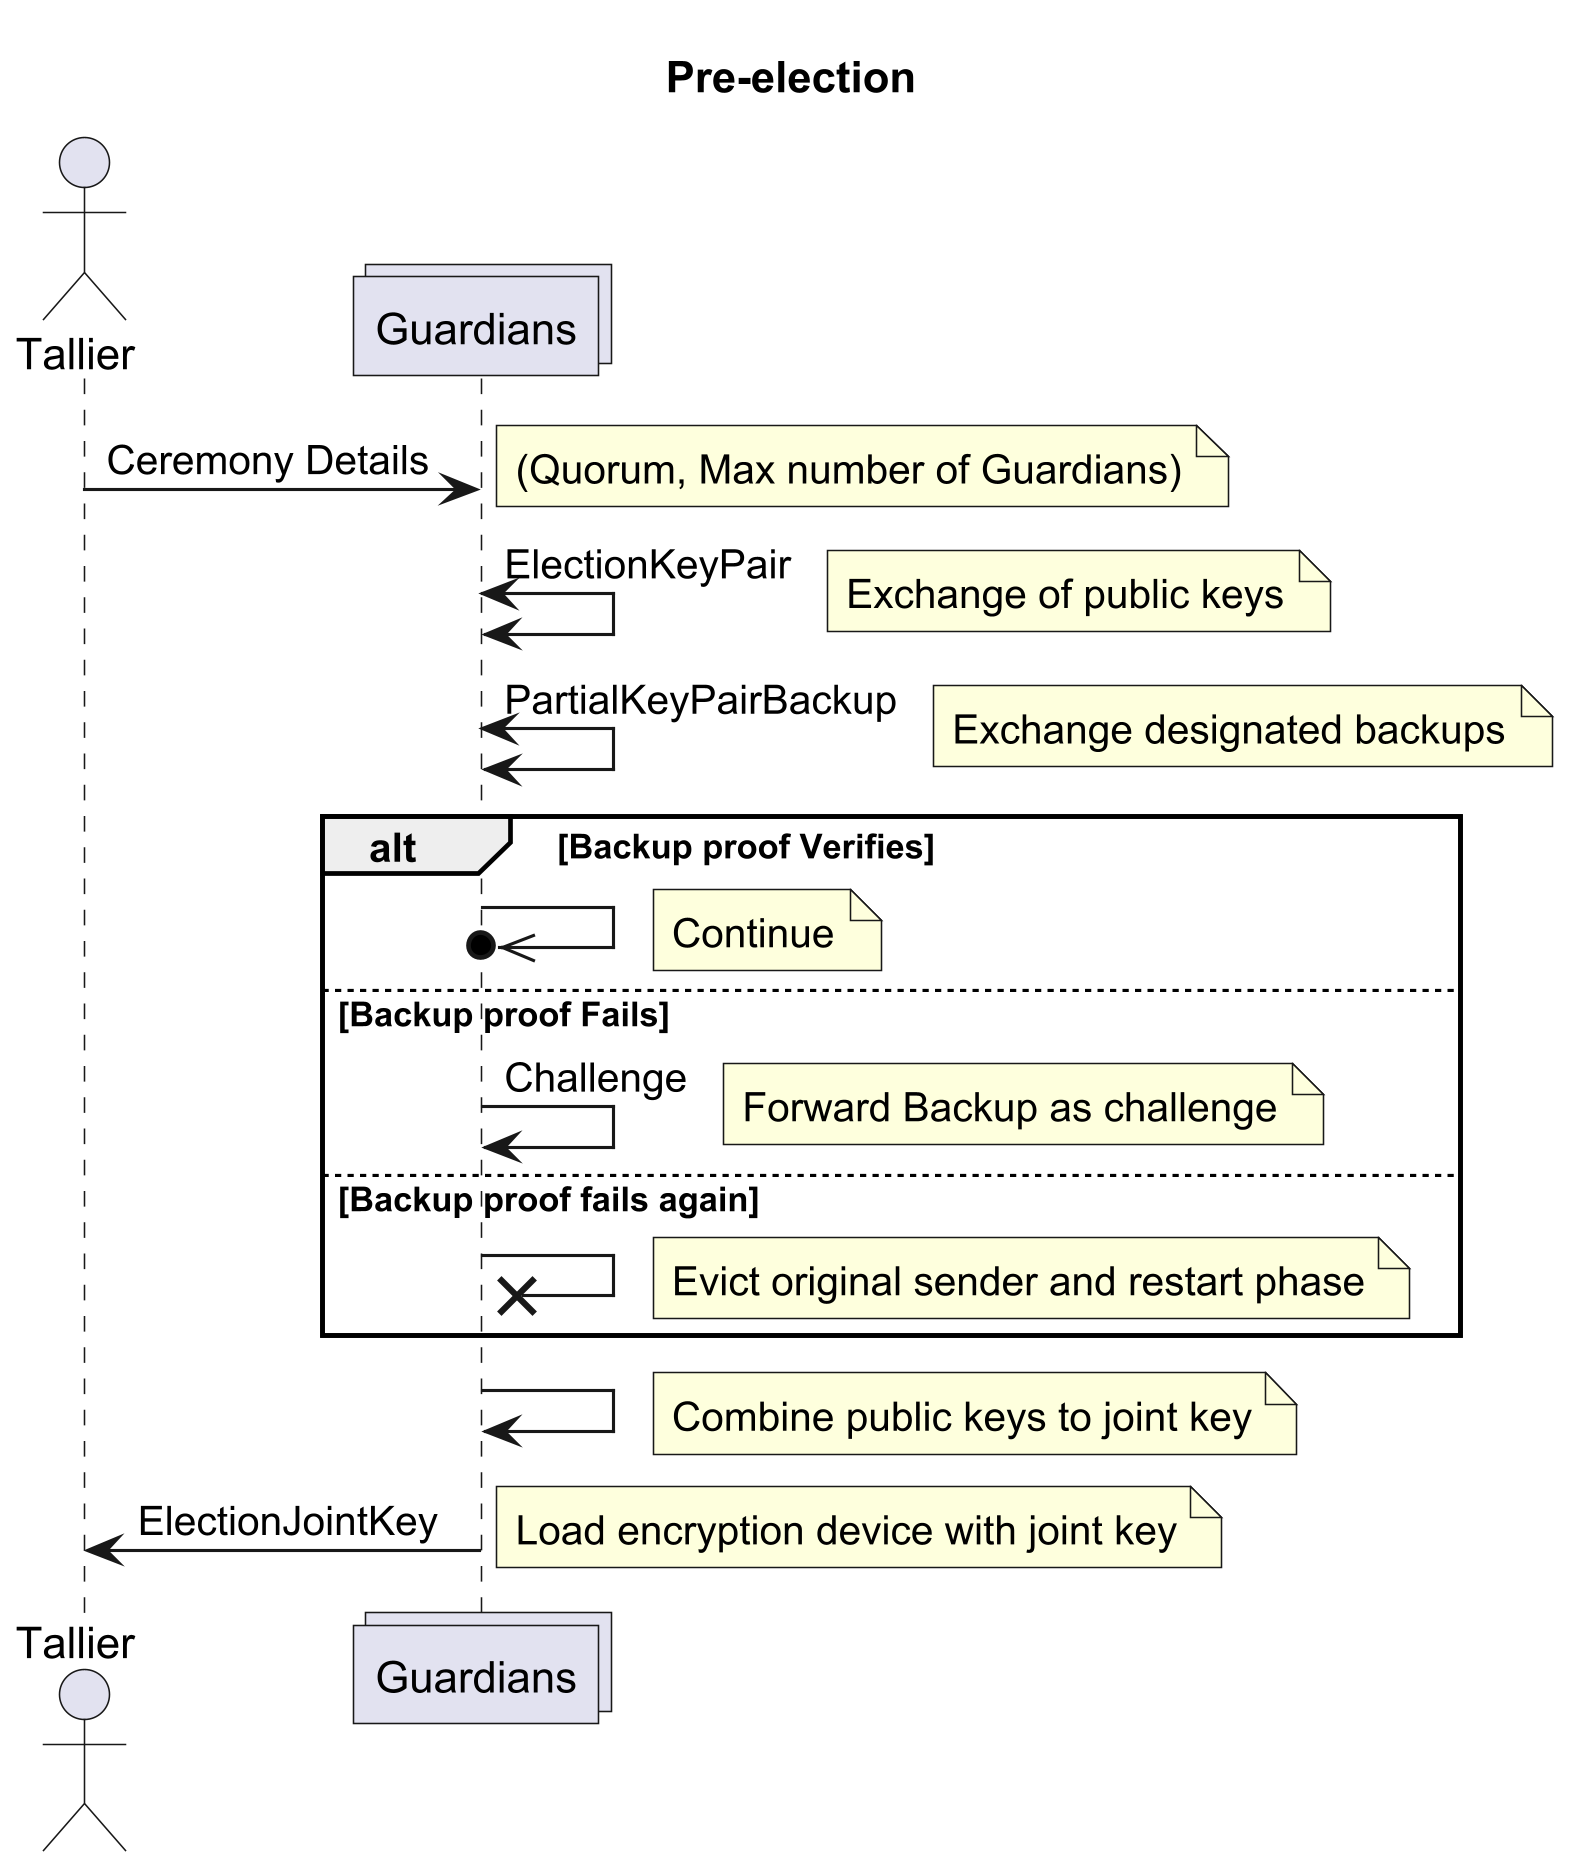
\includegraphics[width=\textwidth]{abbildungen/Diagramme/communication-seq0.png}
    \caption{Communication Sequence in the Pre-election phase}
    \label{Fig:comm-pre}
\end{figure}

A sequence diagram of the pre-election steps are seen in \ref{Fig:comm-pre}. In it we see that the Election administrator sends ceremony details to the Guardians and receives a joint key in return. The joint key is then loaded into the encryption devices. In order to generate a joint key each guardian send their public key to a receiving guardians. The receiving guardian generates a designated backup for each guardian. If a guardian receives a designated backup the included proofs are verified. If a proof failed the guardian send the unverified backup to other guardians as a challenge. If the proof fails again this guardian that generated the backup is evicted and the ceremony has to be restarted. 

\begin{figure}
    \centering
    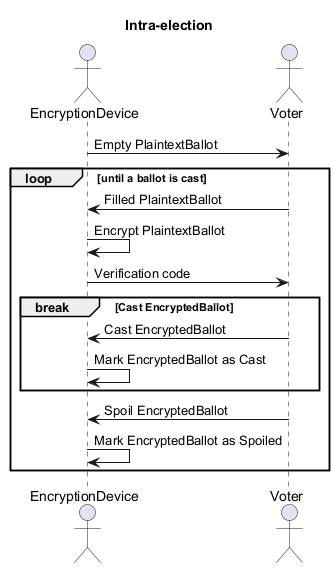
\includegraphics[width=0.5\textwidth]{abbildungen/Diagramme/communication-seq1.png}
    \caption{Communication Sequence in the Intra-election phase}
    \label{Fig:comm-intra}
\end{figure}


A sequence diagram of the intra-election steps is seen in \ref{Fig:comm-intra}. The election administrator would need an empty ballot to the voter. A voter then sends their filled ballot to the encryption device. The encryption devices sends back a verification code. The voter can then decide to either cast or spoil the ballot associated with the verification code. If the voter decides to spoil the ballot the encryption devices needs to mark the encrypted ballot as spoiled and the process starts a new. The loop is broken if the voter decides to cast a ballot.

\begin{figure}
    \centering
    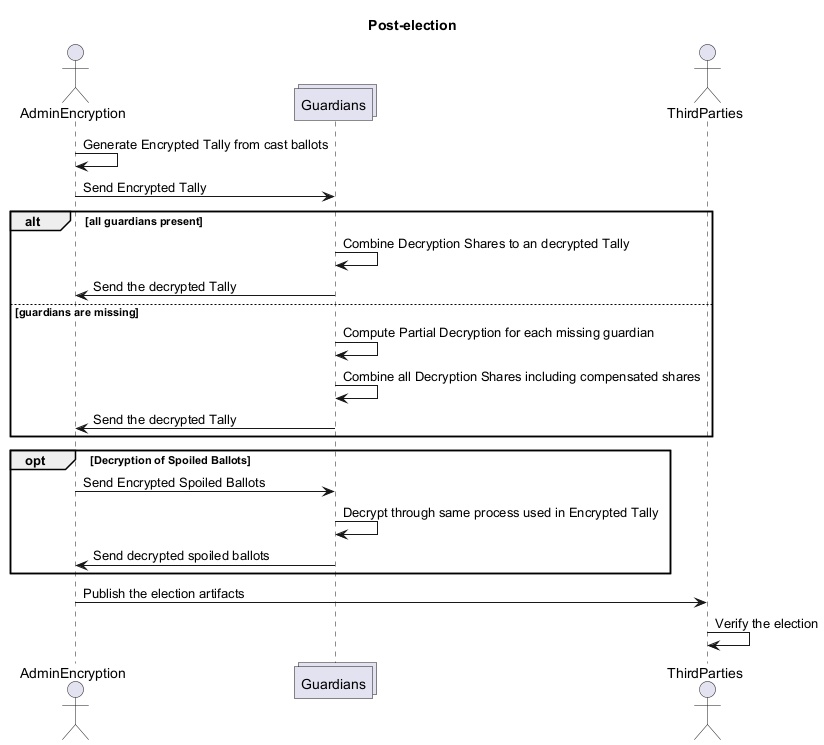
\includegraphics[width=\textwidth]{abbildungen/Diagramme/communication-seq2.png}
    \caption{Communication Sequence in the Post-election phase}
    \label{Fig:comm-post}
\end{figure}

In the post-election steps the encryption device generates a decrypted tally from all cast encrypted ballots and send the encrypted tally to the guardians. If all guardians are present each guardian generates a decryption share which is combined to a decrypted tally. This decrypted tally is then send back to the administrator. If guardians are missing the guardians in addition to generating their decryption share have to compensate for the missing guardians. Missing decryption shares are reconstructed from the backups generated in the pre-election phase. Finally all decryption shares including the reconstructed shares are combined into a decrypted tally. The decrypted tally is then send back to the administrator. Optionally the spoiled ballots can be decrypted through the same mechanisms as the encrypted tally. At the end of the election the administratir publishes all election artifacts to the public for scrutiny.


IoT systems rely primarily on using messaging protocols for exchanging
IoT data and there exists several protocols or frameworks that support distinct types of messaging patterns 
Given that IoT devices typically have limited computational resources and processing power, choosing a
lightweight, reliable, scalable, interoperable, extensible and secure messaging protocol becomes a very
challenging task. \cite[1]{protocols}.


\subsection{Data Link Layer Protocols}
When selecting an appropriate messaging protocol for \ac{IoT} devices, it is essential to consider the hardware characteristics of these devices and the types of data link layer protocols they support. The data link layer is responsible for facilitating data transfers between network entities \cite[1-3]{protocols}. For instance, the ESP32 microcontroller supports both Wi-Fi and Bluetooth data link layer protocols \cite{esp-prog}. The Bluetooth system on the ESP32 can be further divided into Classic Bluetooth and \ac{BLE} \cite{esp-prog} \cite{esp-faq}. Both Wi-Fi and Bluetooth can operate simultaneously, but this requires time-sharing control \cite[77]{esp-faq}.

The throughput of \ac{IoT} devices can vary significantly based on the bandwidth they support. Since there is no universal radio technology for \ac{IoT} devices, the physical data rates they can achieve depend heavily on their size and hardware components cite[1-2]{protocols}. Additionaly, throughout can be influenced by various factors, including environmental interference, connection intervals, and the size of the \ac{MTU} \cite{esp-faq}. The maximum \ac{BLE} throughput achievable on the ESP32 is about 90 KB/s, for Classic Bluetooth is about 200 KB/s, and for Wi-Fi it is about 20 MBit/s TCP and 30 MBits/ UDP \cite[38, 58,71]{esp-faq} \cite[2666]{esp-prog}. 


Wi-Fi (802.11n) generally has a higher transmission range of up to approximately 1 km compared to \ac{BLE}, which has a range of up to approximately 100 m \cite[3]{protocols}. 

Beyond the data link layer protocols, there are networking protocols that operate on top of the \ac{BLE} and Wi-Fi stacks. Both Wi-Fi and \ac{BLE} support mesh networking, which facilitates many-to-many device communication and is optimized for creating large-scale device networks. The Wi-Fi stack also includes the \ac{NAN} protocol, which allows direct device-to-device communication among \ac{NAN} devices without requireing an \ac{AP} connection. However, it is important to note that \ac{NAN} Datapath security is not supported, meaning that data packets cannot be encrypted, making it less suitable for transmitting sensitive information \cite[2694]{esp-prog}. 

Understanding protocols at the data link layer is not sufficient for build IoT applications. It is essential to also consider the protocols that exist at the application level, which complement those at the data link layer. Choosing a protocol that is closer to the application layer while taking into account crucial system requirements- such as \ac{QoS}, bandwidth, interoperability, and security- becomes inevitable \cite[2]{protocols}


\subsection{Application Layer Protocols}
When developing \ac{IoT} systems, choosing the most appropriate
messaging protocols becomes a challenging task. While all messaging protocols facilitate data communication between entities via a transmission medium, their characteristics vary. Understanding how these protocols operate and addressing potential challenges is essential for identifying a suitable protocol. A well-suited messaging protocol can help reduce network traffic and latency, thereby enhancing the reliability of an \ac{IoT} application. For instance, application layer protocols that capture data faster than the actual physical data rates can lead to increased latency. Therefore, it is advisable to consider messaging protocols that can accommodate physical data rates at the data link layer \cite[2,15]{protocols}.

The application layer serves as an abstraction layer \cite[3]{protocols}. Within the ESP32 microcontroller, several application layer protocols address a wide range of application requirements. Some of the notable application layer protocols available as firmware components of the ESP32 include:

\begin{itemize}
    \item HyperText Transfer Protocol (HTTP) \cite{esp-prog}
    \item Message Queueing Telemetry Transport (MQTT) \cite{esp-prog}
    \item Modbus (primarily used in industrial IoT environments)\cite[3]{protocols} \cite{esp-prog}
    \item ESP-NOW (a proprietary protocol for ESP32 devices) \cite{esp-prog}\cite{esp-prog}
\end{itemize}

Each protocol offers various features that differ in terms of reliability, quality of service, performance, functionality, and scalability, among other factors \cite[3]{protocols}. 

\subsection{Payload Size}
One important aspect that narrow down the choice of messaging protocols is the maximum payload size.

The proof sizes play a significant role in the choice of messaging protocols in our IoT application.
At the post-election phase each guardian produces a Chaum-Pedersen proof of correct decryption \cite[15]{eg-paper}.
A Chaum-Pedersen proof contains the following values:
\begin{itemize}
    \item commitment(pad,data): 1024 bytes (standard parameters) or 768 bytes (reduced parameters)
    \item challenge: 32 bytes
    \item response: 32 bytes
\end{itemize}
A Chaum-Pedersen proof to proof a decryption share generated by a guardian is thus 1088 bytes (standard parameters) or 960 bytes (reduced parameters) in size.

During pre-election to ensure robustness and handle missing guardians at the post-election phase, ElectionGuard uses a key generation process that involves sharing private keys among guardians. This allows a Quorum of guardians to decrypt the election results without needing to reconstruct the private keys of missing guardians. These shares are accompanied by Schnorr proofs too ensure the receiving guardians can confirm the shares they receive are meaningful \cite[9]{eg-spec}. 
A Schnorr proof contains the following values:
\begin{itemize}
    \item commitment: 512 bytes (standard parameters) or 384 bytes (reduced parameters)
    \item challenge: 32 bytes
    \item response: 32 bytes
\end{itemize}
A Schnorr proof is thus 576 bytes (standard parameters) or 448 bytes (reduced parameters) in size. If the Quorum is 3 guardians, each guardian would need to generate 3 Schnorr proofs for each guardian. The total size of Schnorr proofs for a Quorum of 3 guardians is 1728 bytes (standard parameters) or 1344 bytes (reduced parameters).


The maximum packet size for the mesh networking technologies is 384 bytes for \ac{BLE} and 1456 bytes for Wi-Fi \cite[35,54]{esp-faq}. A \ac{BLE} network is not suitable for the proposed voting system as the maximum payload size for a Chaum-pedersen proof using reduced parameters is 960 bytes. A Wi-Fi mesh would have trouble with a Quorum of 3 guardians as the maximum payload size for the Schnorr proofs using reduced parameters is already 1344 bytes and this does not include any additional data that needs to be transmitted. The \ac{NAN}. The maximum packet sizes for the Application protocols ESP-NOW is 250 bytes, MQTT is 265 MB and HTTP does not have a limit on the message size \cite[47]{esp-faq} \cite[16]{protocols}.

\subsection{Message Reliability}
\ac{IoT} systems are driven by \ac{IoT} devices that are typically resource-constrained having limited power, networking and processing capabilities. Messaging protocols need to be optimized such that they require minimal resources (e.g. processing power, memory, storage, network bandwidth) which are often needed by IoT devices when communicating data. To this extent, it is imperative that the messaging protocols employed in IoT systems maintain high-levels of quality for data transmission. \cite[15]{protocols}. An IoT system may require that messages be delivered in a reliable manner where all clients acknowledge the receipt of these messages \cite[11]{protocols}. MQTT uses three levels of message transmission reliability, each representing a different level of \ac{QoS} \cite[12]{serialisation}:
\begin{itemize}
    \item \textbf{QoS 0 (most once):} Messages arrives at the receiver either once or not at all \cite[11]{serialisation}
    \item \textbf{QoS 1 (least once):} Ensures that a message arrives at the receiver at least once \cite[11]{serialisation}
    \item \textbf{QoS 2 (exactly once):} Ensures that a message arrives at the receiver exactly once without duplication \cite[11]{serialisation}
\end{itemize}

As the QoS level increases, the reliability of messages’ delivery also increases. However, this also increases the overhead associated with ensuring that all clients receive the intended messages. The more clients are subscribed to receive a message with QoS 2, for example, will increase the overhead on the message broker while ensuring the delivery of the message without duplication or
retransmission. \cite[11]{protocols}.

\subsection{MQTT}
MQTT is designed for constrained environments with low bandwidth. MQTT overs several benefits over HTTP such as asynchronous messaging, lower power consumption, and Quality of Service support \cite[23, 27]{protocols}. 

MQTT uses a publish/subscribe model and is composed of a broker and clients. In this model, clients (publisher) publish messages to a broker via a specific topic. Then, the broker filters these incoming messages and distributes them to to clients (subscriber) who are interested in receiving these messages. To this extent, a client that is interested in receiving these messages must first subscribe to this specific topic. In short, a publisher can send messages to a number of subscribers with one single publish operation to the broker. The broker handles the "broadcasting" or sending messages to all subscribers subscribed to topic of the message. \cite[10]{protocols} \cite[12]{serialisation}. 

Figure \ref{fig:comm-pre-mqtt} shows the communication sequence in the pre-election phase using MQTT.Figure \ref{fig:comm-intra-mqtt} shows the communication sequence in the intra-election phase using MQTT. Figure \ref{fig:comm-post-mqtt} shows the communication sequence in the post-election phase using MQTT. All figures shows a high-level overview of the MQTT brokering model that shows all of the entities involved in this architecture including: (a) centralized broker, (b) publishers and (c) subscribers.  

The further publishers and subscribers are from the broker, the longer the travel time of the MQTT messages and the higher the latency \cite[20]{protocols}. Subscribers can receive published messages at different times. Some studies found that the throughput in MQTT drops significantly as the number of clients’ subscriptions increases. As more clients subscribe to topics the number of messages increases \cite[19,21,22]{protocols}.

\subsection{Data serialization}
Data serialization is the process of structuring data into a streamlined format before storing or transmitting it. Broadly speaking, there are two approaches to serialization: text-based and binary. In text-based serialization, data is typically structured into key-value pairs in a readable text format. In binary serialization, key-value pairs are stored in a binary format, which typically reduces space requirements \cite[11]{serialisation}. The design specification of ElectionGuard does not specify serialization methods or data structures. However, every implementation of ElectionGuard should be compatible with other implementations \cite[23]{eg-paper}. The Python implementation expects data to be serialized into the text-based JSON format.

Exchanging data in different formats across IoT devices raises syntactic interoperability issues that need to be addressed \cite[17]{protocols}. However, if we want to transmit data through the network faster, smaller data sizes are preferable. Additionally, the data does not need to be human-readable during transmission like with text-based formats \cite[225]{protobuffer}. Binary formats are typically preferred as they provide smaller message sizes compared to text-based formats like JSON \cite[11]{serialisation}. For instance, in a test using ESP32, the encoding size was, on average, smaller for Protocol Buffers (a binary format) compared to the text-based JSON format \cite[15]{serialisation-comparison}. Thus we could use a binary format for sending data over the network to reduce the message size however we would need to convert the data into a JSON format for the Python implementation. 

Another benefit of more efficient formats is improved serialization and deserialization speeds. This indicates that fewer CPU cycles are used for data processing, leading to lower power consumption. In one test on the ESP32, the serialization and deserialization speed was almost halved when using Protocol Buffers compared to JSON \cite[11-12]{serialisation-comparison}. 

In our case, choosing a binary serialization approach could be beneficial. The in-memory data representation of our data structures in the ESP32 implementation uses structs, as seen in Appendix \ref{lst:structures}. These structures contain a custom data type, sp\_int, which is a large integer representation. To parse the large integer into a hexadecimal JSON string, we would need to convert each byte of the large integer into a hex representation. In contrast, parsing into a binary format involves simply copying the bytes directly into the output array, which is a more efficient operation.

Our implementation, therefore, chooses Protocol Buffers as the serialization format. A Protocol Buffer implementation is already included in the ESP32 as a component. A significant advantage of Protocol Buffers is that we only need to define the structure for the data to be transferred once and can then exchange it over a wide variety of channels. The programming language is secondary since Protocol Buffers are language-neutral \cite[224]{protobuffer}. Thus, with our .proto files, as seen in Appendix \ref{pre-election}, we can generate code for both the ESP32 and the Python client, as seen in Appendices \ref{lst:generated-c} and \ref{lst:generated-python}. An example of serialising ElectionPartialKeyPair which is the backup shared with other guardians is seen in Appendix \ref{lst:serialize} an example of deserialisation is seen in Appendix \ref{lst:deserialise}. 

\section{Security}
Furthermore,
IoT devices are generally used by humans which makes them
vulnerable to intruders that attempt to gain unsolicited access
or collect confidential personal data in a malicious manner.
\cite[23]{protocols}

An IoT
communication protocol needs to ensure that only authorized
users regardless if they are publishers or subscribers
Furthermore, such vulnerabilities may occur when
offering QoS level 2 which may explain why many IoT cloud
providers not to provide support at this level as presented in
Table VII. 
Although each protocol provides different levels of
security measure\cite[23]{protocols}


The MQTT handling of disallowed Unicode code points
provides a client or server the option to decide on the
validation of these code points (e.g. UTF-8 encoded strings).
As a result, an endpoint does not necessarily need to validate
UTF-8 encoded strings (e.g. topic name or property). As
such, a client could potentially use this as a vulnerability and
causes a subscribed client to close the network connection
using a topic that contains an invalid Unicode code point. A
malicious client can then use this as a security exploit for
possibly causing a Denial of Service (DoS) attack.
Therefore, enabling UTF-8 encoded strings, for example,
can allow these security exploits to occur in cases they are
used as control characters or in control packets (see the first
\cite[11]{protocols}

lack of encryption; can use TLS/SSL for security and
encryption, however, extra connection overhead \cite[27]{protocols}

The case can become worse if the broker’s resources are maximized
and hence a broker can be a Single Point of Failure (SPoF) \cite[19]{protocols}.

\begin{comment}
    Abkürzungen müssen im Abkürzungsverzeichnis angelegt werden.
Erste Verwendung einer \ac{ABK} jede weitere Verwendung der \ac{ABK}.
[5546:2025-02-24 10:38:36,150]:WARNING:chaum_pedersen.py.is_valid:#L233: found an invalid Chaum-Pedersen proof: {'in_bounds_alpha': True, 'in_bounds_beta': True, 'in_bounds_k': True, 'in_bounds_m': True, 'in_bounds_a': True, 'in_bounds_b': True, 'in_bounds_c': True, 'in_bounds_v': True, 'in_bounds_q': True, 'same_c': True, 'consistent_gv': False, 'consistent_av': False, 'k': 'D32530DA334FA7F131BB39D8D69D8AB75CE2ACB5865FF710F583A489C0DC639237A98E5E68DF6B2A7499AB1F1DDB5B88575C2A296DC223997D404B4B6E73237CD9FF9EBB26D9FCD08E040F2DC81E8667FAA31B91B235AEB49FE1529BEE2107D864004C533E52962F5CDD6CBC240F4C7DBEAAD6E4F374C23730D63657F3F9333A51C2C6911951F5B7C2EF7FA04D8EAB27C7B34E7083FD9F96DCC67DF0B0990B4363615EB3173EBBC2F261F30DE98D51696F927BB208A837CC0311395CFC268DFCE2EE4C90E86F8AE0650EB7B842E39D707154E60E46D48CD47954BC401F0A12F36798772EE148BFF1873C445FD59D0D96825A637D64942B06CE5497E56B9F7DDA9C5263506BE999638A76412EF57432AF45310831C4996307BF52FF07FB6FFC401F514C239E273734F3B553C7A2B4555DD0025BCC022DEA511A9AF7A779FDBE66BD2E81695541B2F9DF225FDAD26C18A9C822C23463E210ADA1FF369A49AA4BC94C0778D3810380573B9E8EF815A2F1DE85C14527B714AA97C78423E3634AA662', 'q': '942C2F7FA0926674D1F18D0B4C3AA7F330A5AE0EB23C3F433884C5C06CB5A8FF', 'proof': ChaumPedersenProof(pad='2C14DDC7B799642BF06DB8D96B1B5CA7C8E836804DD74B440CB29A016C58C93B0ED5EDD3BE6B8242493C9723D5F60192DC3B0022FC4A0030932440D1375546D9A4CC41E642DDB1FDC9758ADEC5208DCFDF72A7AB0E70C50AFB3F858DA3FC2F8D3ED372E630A3E344CEA3BA7932845024476D9DFE4FF2CC4AA42FB682911809DCC9A1B9A3DBEF00261F479ED606B001180374A2542ADE378E6D533F76A80D088AF5965D1D6526C4E5FDB6086261130F4577DFDC894E7466E60C3295F83750DEBACE1C3C6FC147524BC5A0EE0E197A4F3A89BFDBAC1DBA7B4CADE7DD0429AA140589437C84424303E637E653EDB3B41105DE6B2D4527E75E2021527D379BEFD2E63F5221558D440DE035E893CB7FC5700BA7831C2B93924B1047E1CEC646917515CB8BBBC67DC4A95A87E288B4EE623EE7CF7BF8545E596467A4F85740BB3B2DBA97F69936379E9A0DA2DA9535ACB3447A755E167FCAE840EB97F3C0BCB9C92380846C279CFA2C6193AD94FA9AEBB1DCA851D1233D4247CAFD09DC227197EF26F8', data='9C37A4AAB9C2FE1839F332EF792CE36DBED2AB532422C66F265BCFEAF3BA76DDEA31C28A0301E34B42B4893CDB5E46C6ED90B859A060893B573A46C8CF4010F178A54436D2EC3DA589B47AF80C6516C7F4BD910C5798919F13ECD45A0209D51F93F326D63C1F82A01910CA6C61086A31AB67ED1E968DDE754E4799163823E48CC44093739312EC8204B804435D66F8EA698D9979FCAB3403DAAB19D12C438576B3A34847E0C06ED91A268491C117DA4CF1892952BD4278AF6B05681D0189E636BB9391B5253584949F7B4749D3BACA8D7F5FA2E224D50940E7590413C099CB36A076B1BE4A3A1AF52E428176479B2EA8C0B15D5CCAA0D33737711BD24DA626AD91B9DFEB34B4B1F5E053CE7C418F1DF601028E2AF1479EE725F109F05E5BF53ECDB8C1C362C957C1AC6E5E95A72DAC4120B84D0A149A6A4BE641D0BA4C7D515FB181CEF22C05DE344E7A124BB48F23644FF70A667A57BA0BA9E0C69479D3FA01CC089397F74B413E2DA69A5AAA1B3DD08E1B9A83F8911D3C9811EF12F5148F07', challenge='42D5BED6EDF3B7299974309A842A9831799F8204AA4BDDE73C1E95B7C250E7DC', response='0EFDF49FAC6B36D6817132E6AA2723A76CAAC7905D6489325FECC0A0DC817211', usage=<ProofUsage.SecretValue: 'Prove knowledge of secret value'>)}
[5546:2025-02-24 10:38:36,167]:WARNING:decryption_share.py.is_valid:#L129: CiphertextDecryptionSelection is_valid failed for guardian: 083af2b6253c selection: yes-selection with invalid proof
[5546:2025-02-24 10:38:36,178]:WARNING:decrypt_with_shares.py.decrypt_selection_with_decryption_shares:#L182: share: yes-selection has invalid proof or recovered parts
[5546:2025-02-24 10:38:36,188]:WARNING:decrypt_with_shares.py.decrypt_contest_with_decryption_shares:#L146: could not decrypt contest referendum-single-vote with selection yes-selection
[5546:2025-02-24 10:38:36,200]:WARNING:decrypt_with_shares.py.decrypt_tally:#L66: contest: referendum-single-vote failed to decrypt with shares

\end{comment}


%Befehl um sämtliche Literatur im Literaturverzeichnis aufzuführen
\nocite{*}

